\documentclass[a4paper, 11pt]{article}

\usepackage{amsmath}
\usepackage{amssymb}
\usepackage{geometry}
\usepackage{natbib}
\usepackage{graphicx}
\usepackage[utf8]{inputenc}
\usepackage{tikz}
\usepackage[most]{tcolorbox}
\usepackage[backref=page]{hyperref}


\definecolor{antiquewhite}{rgb}{0.98, 0.92, 0.84}

\newtcbtheorem{Takeaway}{\bfseries Takeaway}{enhanced,
  coltitle=black,
  top=0.3in,
  colback=antiquewhite,
  attach boxed title to top left=
  {xshift=1.5em,yshift=-\tcboxedtitleheight/2},
  boxed title style={size=small,colback=pink}
}{Takeaway}

\geometry{left=1.5cm, top=1.5cm, right=1.5cm, bottom=2cm, footskip=.5cm} 
%dvips -Ppdf -tletter -G0 -o paper.ps paper.dvi


\newcommand{\A}{\mathbb{A}}
\newcommand{\B}{\mathbb{B}}
\newcommand{\C}{\mathbb{C}}
\newcommand{\D}{\mathbb{D}}
\newcommand{\E}{\mathbb{E}}
\newcommand{\F}{\mathbb{F}}
\newcommand{\G}{\mathbb{G}}
\newcommand{\Hh}{\mathbb{H}} 
\newcommand{\I}{\mathbb{I}}
\newcommand{\J}{\mathbb{J}}
\newcommand{\K}{\mathbb{K}}
\newcommand{\M}{\mathbb{M}}
\newcommand{\N}{\mathbb{N}}
% \newcommand{\P}{\mathbb{P}}
\newcommand{\Q}{\mathbb{Q}}
\newcommand{\R}{\mathbb{R}}
% \newcommand{\S}{\mathbb{S}}
\newcommand{\T}{\mathbb{T}}
\newcommand{\U}{\mathbb{U}}
\newcommand{\V}{\mathbb{V}}
\newcommand{\W}{\mathbb{W}}
\newcommand{\X}{\mathbb{X}}
\newcommand{\Y}{\mathbb{Y}}
\newcommand{\Z}{\mathbb{Z}}


\newcommand{\x}{\times}



%*********For chapter on binary and categorical data***********
\newcommand{\tvx}{\widetilde{\vx}}
\newcommand{\tvX}{\widetilde{\vX}}
\newcommand{\deriv}[2]{\frac{\partial{#1}}{\partial{#2}}}
\newcommand{\secondderiv}[2]{\frac{\partial^2{#1}}{\partial{#2}^2}}
\newcommand{\neglvb}{\overline{f}}
\newcommand{\bv}{\overline{v}}
\newcommand{\bvm}{\overline{\vm}}
\newcommand{\bvv}{\overline{\vv}}
\newcommand{\bvV}{\overline{\vV}}
\newcommand{\tmu}{\widetilde{\vmu}}
\newcommand{\tSigma}{\widetilde{\vSigma}}
\newcommand{\tm}{\widetilde{m}}
\newcommand{\tv}{\widetilde{v}}
\newcommand{\tsigma}{\widetilde{\sigma}}
\newcommand{\tV}{\widetilde{V}}
\newcommand{\tvSigma}{\widetilde{\vSigma}}
\newcommand{\tg}{\widetilde{\gamma}}
\newcommand{\tvm}{\widetilde{\vm}}
\newcommand{\tvv}{\widetilde{\vv}}
\newcommand{\tvV}{\widetilde{\vV}}
\newcommand{\tvLambda}{\widetilde{\vLambda}}
\newcommand{\tvlambda}{\widetilde{\vlambda}}
\newcommand{\tlambda}{\widetilde{\lambda}}
\newcommand{\tvgamma}{\widetilde{\vgamma}}
\newcommand{\tgamma}{\widetilde{\gamma}}
\newcommand{\teta}{\widetilde{\eta}}
\newcommand{\tphi}{\widetilde{\phi}}

\newcommand{\talpha}{\widetilde{\alpha}}
\newcommand{\tvg}{\widetilde{\vg}}
\newcommand{\tvh}{\widetilde{\vh}}
\newcommand{\tvH}{\widetilde{\vH}}
\newcommand{\tvP}{\widetilde{\vP}}
\newcommand{\tvG}{\widetilde{\vG}}
\newcommand{\tvA}{\widetilde{\vA}}
\newcommand{\tp}{\tilde{p}}
%\newcommand{\lse}{\mbox{llp}}
%\usepackage{algorithm}

% numbers a line in align* block
\newcommand\numberthis{\addtocounter{equation}{1}\tag{\theequation}}


%% densify spacing in bibliographies
\newcommand{\bibfix}{%    PUT \bibfix in file.bbl after first line
    \setlength{\parsep}{\parskip}%
    \setlength{\itemsep}{0cm}%
    \setlength{\topsep}{\parskip}%
    \setlength{\parskip}{0cm}%
    \setlength{\partopsep}{0cm}%
    \setlength{\listparindent}{\parindent}%
    \setlength{\labelwidth}{10pt}%
    \setlength{\labelsep}{0pt}%
    \setlength{\leftskip}{0pt}%
    \setlength{\leftmargin}{0pt}%
}


\newtheorem{claim}{Claim}{}
\newtheorem{thm}{Theorem}{}
\newtheorem{prop}{Proposition}{}
\newtheorem{corr}{Corollary}{}
%\newtheorem{lemma}{Lemma}{}
\newtheorem{defn}{Definition}{}
\newenvironment{mythm}{{\bf Theorem}}{}
\newenvironment{myproof}{{\bf Proof}}{}


\newcommand{\choice}[2]{\left(\!\!\! \begin{array}{c} #1 \\ #2\end{array} \!\!\!\right)}
\newcommand{\half}{\mbox{$\frac{1}{2}$}}
\newcommand{\defeq}{\stackrel{\rm def}{=}}
%\newcommand{\defeq}{\mbox{$\stackrel{\rm def}{=}}$}
%\newcommand{\real}{{\rm I\hspace{-0.2em}R}}
\newcommand{\lra}{\mbox{$\leftrightarrow$}}
\newcommand{\Ra}{\mbox{$\Rightarrow$}}
\newcommand{\la}{\mbox{$\leftarrow$}}
\newcommand{\tr}{\mbox{$\mbox{tr}$}}
%\newcommand{\det}{\mbox{$\mbox{det}$}}

\newcommand{\rnd}[1]{\left(#1\right)}
\newcommand{\sqr}[1]{\left[#1\right]}
\newcommand{\crl}[1]{\left\{#1\right\}}
\newcommand{\myang}[1]{\langle#1\rangle}


\newcommand{\range}{\mbox{$\mbox{range}$}}
\newcommand{\myspan}{\mbox{$\mbox{span}$}}
\newcommand{\nullspace}{\mbox{$\mbox{nullspace}$}}
\newcommand{\adj}{\mbox{$\mbox{adj}$}}
\newcommand{\nbd}{\mbox{$\mbox{nbd}$}}



\newcommand{\define}[1]{{\bf #1}}


%\newcommand{\keyword}[1]{{\bf #1}}
\newcommand{\keyword}[1]{{\bf #1}\index{keywords}{#1}}
\newcommand{\addtoindex}[1]{#1 \index{keywords}{#1}}
\newcommand{\keywordSpecial}[2]{{\bf #1}\index{keywords}{#2@#1}}
\newcommand{\bfidx}[1]{{\bf #1}}
\newcommand{\keywordDef}[1]{{\bf #1}\index{keywords}{#1|bfidx}}
%\newcommand{\keyworddef}[1]{{\bf #1}\index{keywords}{#1@{\bf #1}}}
\newcommand{\codename}[1]{{\tt #1}\index{code}{#1}}
\newcommand{\netlabname}[1]{{\tt #1}}
\newcommand{\Rcmd}[1]{{\tt #1}}
\newcommand{\matlabcmd}[1]{{\tt #1}}
\newcommand{\matlabscript}[1]{{\tt #1}}
\newcommand{\dataname}[1]{{\tt #1}}

%\newcommand{\dim}{\mbox{dim}}
\newcommand{\softmax}{\calS}
%\newcommand{\softmax}{\mbox{softmax}}
\newcommand{\sign}{\mbox{sign}}
\newcommand{\iid}{\mbox{iid}}
\newcommand{\mle}{\mbox{mle}}
\newcommand{\myiff}{\mbox{iff}}
\newcommand{\pd}{\mbox{pd}}
\newcommand{\pdf}{\mbox{pdf }}
\newcommand{\cdf}{\mbox{cdf}}
\newcommand{\pmf}{\mbox{pmf}}
\newcommand{\wrt}{\mbox{wrt}}
\newcommand{\MLABA}{\mbox{FML}}
\newcommand{\mywp}{\mbox{wp}}

\newcommand{\myvec}[1]{\mbox{$\mathbf{#1}$}}
\newcommand{\myvecsym}[1]{\mbox{$\boldsymbol{#1}$}}

\newcommand{\vzero}{\mbox{$\myvecsym{0}$}}
\newcommand{\vone}{\mbox{$\myvecsym{1}$}}

\newcommand{\valpha}{\mbox{$\myvecsym{\alpha}$}}
\newcommand{\vbeta}{\mbox{$\myvecsym{\beta}$}}
\newcommand{\vchi}{\mbox{$\myvecsym{\chi}$}}
\newcommand{\vdelta}{\mbox{$\myvecsym{\delta}$}}
\newcommand{\vDelta}{\mbox{$\myvecsym{\Delta}$}}
\newcommand{\vepsilon}{\mbox{$\myvecsym{\epsilon}$}}
\newcommand{\veta}{\mbox{$\myvecsym{\eta}$}}
\newcommand{\vgamma}{\mbox{$\myvecsym{\gamma}$}}
\newcommand{\vmu}{\mbox{$\myvecsym{\mu}$}}
\newcommand{\vlambda}{\mbox{$\myvecsym{\lambda}$}}
\newcommand{\vLambda}{\mbox{$\myvecsym{\Lambda}$}}
\newcommand{\vLambdaBar}{\mbox{$\overline{\vLambda}$}}
\newcommand{\vrho}{\mbox{$\myvecsym{\rho}$}}
\newcommand{\vphi}{\mbox{$\myvecsym{\phi}$}}
\newcommand{\vPhi}{\mbox{$\myvecsym{\Phi}$}}
\newcommand{\vpi}{\mbox{$\myvecsym{\pi}$}}
\newcommand{\vpsi}{\myvecsym{\psi}}
\newcommand{\vPsi}{\mbox{$\myvecsym{\Psi}$}}
\newcommand{\vtheta}{\mbox{$\myvecsym{\theta}$}}
\newcommand{\vTheta}{\mbox{$\myvecsym{\Theta}$}}
\newcommand{\vsigma}{\mbox{$\myvecsym{\sigma}$}}
\newcommand{\vSigma}{\mbox{$\myvecsym{\Sigma}$}}
\newcommand{\vOmega}{\mbox{$\myvecsym{\Omega}$}}
\newcommand{\vtau}{\mbox{$\myvecsym{\tau}$}}
\newcommand{\vxi}{\mbox{$\myvecsym{\xi}$}}

\newcommand{\va}{\mbox{$\myvec{a}$}}
\newcommand{\vb}{\mbox{$\myvec{b}$}}
\newcommand{\vc}{\mbox{$\myvec{c}$}}
\newcommand{\vd}{\mbox{$\myvec{d}$}}
\newcommand{\ve}{\mbox{$\myvec{e}$}}
\newcommand{\vo}{\mbox{$\myvec{o}$}}
\newcommand{\vi}{\mbox{$\myvec{i}$}}
\newcommand{\vf}{\mbox{$\myvec{f}$}}
\newcommand{\vg}{\mbox{$\myvec{g}$}}
\newcommand{\vh}{\mbox{$\myvec{h}$}}
\newcommand{\vj}{\mbox{$\myvec{j}$}}
\newcommand{\vk}{\mbox{$\myvec{k}$}}
\newcommand{\vm}{\mbox{$\myvec{m}$}}
\newcommand{\vn}{\mbox{$\myvec{n}$}}
\newcommand{\vp}{\mbox{$\myvec{p}$}}
\newcommand{\vq}{\mbox{$\myvec{q}$}}
\newcommand{\vr}{\mbox{$\myvec{r}$}}
\newcommand{\vs}{\mbox{$\myvec{s}$}}
\newcommand{\vt}{\mbox{$\myvec{t}$}}
\newcommand{\vu}{\mbox{$\myvec{u}$}}
\newcommand{\vv}{\mbox{$\myvec{v}$}}
\newcommand{\vw}{\mbox{$\myvec{w}$}}
\newcommand{\vws}{\mbox{$\vw_s$}}
\newcommand{\vwh}{\mbox{$\hat{\vw}$}}
\newcommand{\vx}{\mbox{$\myvec{x}$}}
\newcommand{\vxt}{\mbox{$\myvec{\tilde{x}}$}}
\newcommand{\vy}{\mbox{$\myvec{y}$}}
\newcommand{\vyt}{\mbox{$\myvec{\tilde{y}}$}}
\newcommand{\vz}{\mbox{$\myvec{z}$}}
\newcommand{\vA}{\mbox{$\myvec{A}$}}
\newcommand{\vB}{\mbox{$\myvec{B}$}}
\newcommand{\vC}{\mbox{$\myvec{C}$}}
\newcommand{\vD}{\mbox{$\myvec{D}$}}
\newcommand{\vE}{\mbox{$\myvec{E}$}}
\newcommand{\vF}{\mbox{$\myvec{F}$}}
\newcommand{\vG}{\mbox{$\myvec{G}$}}
\newcommand{\vH}{\mbox{$\myvec{H}$}}
\newcommand{\vI}{\mbox{$\myvec{I}$}}
\newcommand{\vJ}{\mbox{$\myvec{J}$}}
\newcommand{\vK}{\mbox{$\myvec{K}$}}
\newcommand{\vL}{\mbox{$\myvec{L}$}}
\newcommand{\vM}{\mbox{$\myvec{M}$}}
\newcommand{\vN}{\mbox{$\myvec{N}$}}
\newcommand{\vO}{\mbox{$\myvec{O}$}}
\newcommand{\vP}{\mbox{$\myvec{P}$}}
\newcommand{\vQ}{\mbox{$\myvec{Q}$}}
\newcommand{\vR}{\mbox{$\myvec{R}$}}
\newcommand{\vS}{\mbox{$\myvec{S}$}}
\newcommand{\vT}{\mbox{$\myvec{T}$}}
\newcommand{\vU}{\mbox{$\myvec{U}$}}
\newcommand{\vV}{\mbox{$\myvec{V}$}}
\newcommand{\vW}{\mbox{$\myvec{W}$}}
\newcommand{\vX}{\mbox{$\myvec{X}$}}
%\newcommand{\vXs}{\mbox{$\vX_{\vs}$}}
\newcommand{\vXs}{\mbox{$\vX_{s}$}}
\newcommand{\vXt}{\mbox{$\myvec{\tilde{X}}$}}
\newcommand{\vY}{\mbox{$\myvec{Y}$}}
\newcommand{\vZ}{\mbox{$\myvec{Z}$}}



\newcommand{\precw}{\mbox{$\lambda_{w}$}} % precision of weights (alpha)
\newcommand{\precy}{\mbox{$\lambda_{y}$}} % precision of y (beta)
\newcommand{\fbar}{\mbox{$\overline{f}$}}
\newcommand{\xbar}{\mbox{$\overline{x}$}}
\newcommand{\ybar}{\mbox{$\overline{y}$}}
\newcommand{\vxbar}{\mbox{$\overline{\vx}$}}
\newcommand{\vybar}{\mbox{$\overline{\vy}$}}
\newcommand{\Xbar}{\mbox{$\overline{X}$}}
\newcommand{\Ybar}{\mbox{$\overline{Y}$}}
\newcommand{\Jbar}{\mbox{$\overline{J}$}}
\newcommand{\Lbar}{\mbox{$\overline{L}$}}
\newcommand{\Tbar}{\mbox{$\overline{T}$}}

\newcommand{\htilde}{\mbox{$\tilde{h}$}}
\newcommand{\vhtilde}{\mbox{$\tilde{\vh}$}}
\newcommand{\Dtilde}{\mbox{$\tilde{D}$}}
\newcommand{\wtilde}{\mbox{$\tilde{w}$}}
\newcommand{\xtilde}{\mbox{$\tilde{x}$}}
\newcommand{\Xtilde}{\mbox{$\tilde{X}$}}
\newcommand{\ytilde}{\mbox{$\tilde{y}$}}
\newcommand{\Ytilde}{\mbox{$\tilde{Y}$}}
\newcommand{\vxtilde}{\mbox{$\tilde{\vx}$}}
\newcommand{\vytilde}{\mbox{$\tilde{\vy}$}}
\newcommand{\ztilde}{\mbox{$\tilde{\z}$}}
\newcommand{\vztilde}{\mbox{$\tilde{\vz}$}}
\newcommand{\vthetaMAP}{\mbox{$\hat{\vtheta}_{MAP}$}}
\newcommand{\vthetahat}{\mbox{$\hat{\vtheta}$}}
\newcommand{\thetahat}{\mbox{$\hat{\theta}$}}
\newcommand{\thetabar}{\mbox{$\overline{\theta}$}}
\newcommand{\vthetabar}{\mbox{$\overline{\vtheta}$}}
\newcommand{\pibar}{\mbox{$\overline{\pi}$}}
\newcommand{\vpibar}{\mbox{$\overline{\vpi}$}}


\newcommand{\sss}{\mbox{$s^2$}}
\newcommand{\vvv}{\mbox{$v$}}
\newcommand{\RSS}{\mbox{RSS}}

%\newcommand{\do}{\mbox{$\mbox{do}$}}

%\newcommand{\xdi}{\mbox{$x_{di}$}}
%\newcommand{\xji}{\mbox{$x_{ji}$}}
%\newcommand{\yi}{\mbox{$y_i$}}



\newcommand{\ki}{i}
\newcommand{\kj}{j}
\newcommand{\kk}{k}

\newcommand{\kC}{C}
\newcommand{\kc}{c}
\newcommand{\calA}{\mbox{${\cal A}$}}
\newcommand{\calC}{\mbox{${\cal C}$}}
\newcommand{\calD}{\mbox{${\cal D}$}}
\newcommand{\calDx}{\mbox{${\cal D}_x$}}
\newcommand{\calE}{\mbox{${\cal E}$}}
\newcommand{\calF}{\mbox{${\cal F}$}}
\newcommand{\calG}{\mbox{${\cal G}$}}
\newcommand{\calH}{\mbox{${\cal H}$}}
\newcommand{\calHX}{\mbox{${\cal H}_X$}}
\newcommand{\calHy}{\mbox{${\cal H}_y$}}
\newcommand{\calI}{\mbox{${\cal I}$}}
\newcommand{\calK}{\mbox{${\cal K}$}}
\newcommand{\calM}{\mbox{${\cal M}$}}
\newcommand{\calMp}{\mbox{$\calM^+$}}
\newcommand{\calMm}{\mbox{$\calM^-$}}
\newcommand{\calMo}{\mbox{$\calM^o$}}
\newcommand{\Ctest}{\mbox{$C_*$}}
\newcommand{\calP}{\mbox{${\cal P}$}}
\newcommand{\calS}{\mbox{${\cal S}$}}
\newcommand{\calSstar}{\mbox{$\calS_*$}}
\newcommand{\calT}{\mbox{${\cal T}$}}
\newcommand{\calV}{\mbox{${\cal V}$}}
\newcommand{\calX}{\mbox{${\cal X}$}}
\newcommand{\calY}{\mbox{${\cal Y}$}}




\usetikzlibrary{quotes, positioning}

\title{Notes of Deep Diffusion Models}
\author{Anand Subramanian}
\date{}

\begin{document} 
\maketitle

\tableofcontents


Energy-based Models (EBMs) are a general class of models for learning probability densities. For some arbitrary probability density $p(\vx)$ for $\vx \in \R^D$, we can express it in a parametric form as

\begin{align}
p(\vx) &= \frac{\exp \left(-E_\theta(\vx)\right)}{Z(\theta)}; \qquad Z(\theta) = \int \exp \left (-E_\theta(\vx) \right) d\vx && \eqcomment{EBM}
\end{align} 

Where $E_\theta: \R^D \to \R$ is the \textit{energy function} and $Z(\theta)$ is the normalizing constant to yield a proper probability density. The energy function is parameterized by $\theta$ can learn to map the given samples $\vx$ to a scalar value following the actual probability density. The learning problem is then to estimate the parameters $\theta$ such that the distribution $p_\theta(\vx)$ estimated by the above EBM converges to the target distribution $p(\vx)$.

The issue with EBMs when it was originally proposed by \cite{lecun2006tutorial} is that the normalizing constant $Z$ (sometimes called as the \textit{partition function}) is intractable for any remotely interesting distribution. The modern developments since then, have largely been to model to densities using the energy function, entirely ignoring the normalizing constant.

The score function is invariant to scaling. 
\begin{align}
    \nabla_{\vx} \log \tilde{p}(\vx) = \nabla_{\vx} \log \left ( p(\vx) Z \right ) = \nabla_{\vx} \left (  \log p(\vx) + \log Z \right ) = \nabla_{\vx} \log  p(\vx)
\end{align}
Therefore, the score function can be used even if we only have the unnormalized density $\tilde{p}(\vx)$. 

This is why people moved away from maximizing (log-) likelihood to optimizing the score function. THis make it ubiquitous in injective flows, and EBMs.


The fundamental idea is to use the \emph{score function} of the above parametric distribution, defined as 

\begin{align}
    \frac{\partial \log p_\theta(\vx)}{\partial \theta} = \E 
\end{align}


\section{Generative Modelling via Probability Density Estimation}

If you can sample from a probability density, then you know the density.

\subsection{Impossibility of Probability Density Estimation}
Impossibility of even conditional probability estimation.

\section{Probability Flows}
In probability theory, the change of variables (CoV) formula is one of the fundamental formulas, which describes how probability density functions relate under a smooth invertible transformation $-$ think coordinate transformation but for random variables. Say we have a random variable $\vx \sim p(\vx)$ and an invertible differentiable transformation $f: \R^D \to \R^M$ defined as $\vy = f(\vx)$, then the resultant random variable $\vy$ follows the density given by
\begin{align}
    \vy \sim q(\vy) = p\left(f^{-1}(\vy) \right)\left |\det \vJ_{f^{-1}} \right|; \qquad \vJ_{f^{-1}} = \frac{\partial f^{-1}(\vy)}{\partial \vy} \in \R^{D \x M}
\end{align}
Where $\vJ_{f^{-1}}$ is the Jacobian of the inverse function $f^{-1}$. Since the transformation is invertible, we can also construct the reverse CoV formula as

\begin{align}
    \vx \sim p(\vx) = q\left(f(\vx) \right)\left |\det \vJ_{f} \right|; \qquad \vJ_{f} = \frac{\partial f(\vx)}{\partial \vx} \in \R^{M \x D}
\end{align}
Where $\vJ_{f}$ is the Jacobian of the transformation $f$. The absolute determinant of the Jacobian $\left |\det \vJ_{f} \right|$quantifies the relative change of volume over a small neighborhood around $\vx$ due to the transformation $f$. Geometrically, the space $\R^D$ is warped by the transformation $f$ to mold $p(\vx)$ into $q(\vy)$.

The transformation function $f$, also called \emph{flow}, has no limitation except that it should be differentiable and invertible. Based on this, we can construct few classes of transformations or flows based on different characteristics such as stochasticity, compression, composability, etc \citep{kothe2023review}.


\subsection{Bijective Flows}
Bijective flows are deterministic transformation between the random variables $\vx, \vy$. As the name suggests, the transformation preserves the dimensions $f: \R^D \to \R^D$ of the random variables. Consequently, $\vJ_{f}, \vJ_{f^{-1}} \in \R^{D \x D}$. An important implication is that the resulting density $q(\vy)$ is properly normalized as normalization factor for each dimension is given by the Jacobian. Thus, Bijective flows are also called \emph{Normalizing Flows} (NF) \citep{papamakarios2021normalizing}. 

\subsubsection{Invertible ResNets as Bijective Flows}


\subsubsection{Incompressible Flows}
A special case of Bijective flows are the class of \emph{incompressible flows}, where $\det \vJ_f = \det \vJ_{f^{-1}} = 1$. Recall the geometric interpretation of Jacobian as the volumetric scaling matrix. When determinant is the same between the transformations, when the "volume" is preserved, and hence flows are incompressible flows. 

Fourier Transforms, PCA are Incompressible flows. 

VQ Flows (assignment), GMM-flows (soft assignment)


\subsection{Injective Flows}
Injective flows are deterministic transformations where the dimensions are not preserved. The random variables $\vx \in R^D$ and $\vy \in \R^M$ can be of different dimensions and as such the resulting PDF is generally unnormalized. Note that injective transformations are still invertible. Interestingly, in this context, one may view the (forward) transformation $f$ as an \emph{encoder} that encodes $\vx$ from one domain to another. The inverse transformation $f^{-1}$ is called as a \emph{decoder}.


Composition of injective functions is injective.


\subsection{Stochastic Flows}
Stochastic flows are transformations where the source variable $\vx$ are mapped stochastically to the target variable $\vy$ \emph{conditioned} on $\vx$. The transformation $f$ can be viewed as a stochastic encoder mapping the source distribution to a conditional distribution.

\begin{align}
    \vy \sim p(\vy | \vx)
\end{align}

To get the inverse flow of the above equation, we observe that the flow must preserve the joint density $p(\vx, \vy)$ for self consistency.

\begin{align}
    p(\vx, \vy) = p(\vx)p(\vx | \vy) = p(\vy)p(\vy|\vx)
\end{align}

The above equation necessitates a stochastic decoder, with the source distribution $p(\vx$) obtained through marginalization over $\vy$.

\begin{align} \label{eq:sto_marg}
    p(\vx)= \E_{\vy \sim p(\vy) } \left [ p(\vx | \vy) \right ] = \int p(\vx | \vy) p(\vy) d\vy
\end{align}

\subsubsection{Markov Flows}

\begin{center} 
    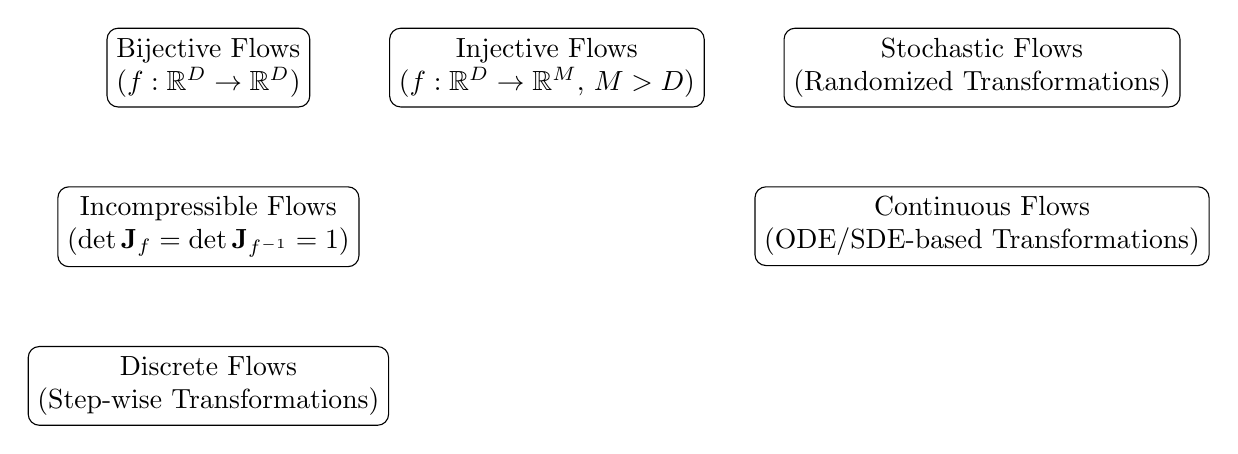
\begin{tikzpicture}[
        every node/.style={draw, align=center, rounded corners, minimum width=2.5cm, minimum height=1cm},
        arrow/.style={->, thick}
    ]
    
    % Nodes
    \node (bijective) {Bijective Flows\\($f: \mathbb{R}^D \to \mathbb{R}^D$)};
    \node [below=of bijective]  (incomp) {Incompressible Flows\\($\det \vJ_f = \det \vJ_{f^{-1}} = 1$)};

    \node[right=of bijective] (injective) {Injective Flows\\($f: \mathbb{R}^D \to \mathbb{R}^M$, $M > D$)};
    \node[right=of injective] (stochastic) {Stochastic Flows\\(Randomized Transformations)};
    \node[below=of incomp] (discrete) {Discrete Flows\\(Step-wise Transformations)};
    \node[below=of stochastic] (continuous) {Continuous Flows\\(ODE/SDE-based Transformations)};
    
    % Arrows
    % \draw[arrow] (bijective) -- (injective);
    % \draw[arrow] (bijective) -- (stochastic);
    % \draw[arrow] (stochastic) -- (discrete);
    % \draw[arrow] (stochastic) -- (continuous);
    % \draw[arrow] (bijective) -- (incomp);

    
    \end{tikzpicture}
\end{center} 


The tipping point for the the Diffusion revolution is to observe that $p(\vx)$ can be a well-defined, easy to sample, easy to model, distribution, while $p(\vy)$ can be an arbitrarily complex distribution, as long as we have a sophisticated transformation $f$ that is smooth and invertible.


Dalton Board as Incompressible flow.

\section{Composing Flows}
Consider the extreme case where the transformation is a vector-to-scalar function $f: \R^D \to \R$. In such case, the CoV formula does not really exist as the transformation can only be specified as a marginalization.

\begin{align} \label{eq:extreme_case}
    q(\vy) = \int p(\vx) \delta (\vy - f(\vx)) d\vx
\end{align}

Where $\delta$ is the Dirac delta function. The above formula essentially says that the target distribution exists only where $\vx$ is mapped onto the real line $\R$ with magnitude $p(\vx)$ \textit{i.e.} the it is a degenerate distribution. In the earlier discussion on the various flows, the use case was be to able to sample from one distribution, transform to another distribution, and back. However, we do not have an inverse for the above equation.
You may observe that the above transformation $f: \R^D \to \R$ is just the energy function $E_\theta(\vx)$ in case of EBMs. In fact, every classifier model is an example of the above case.

Consider a generic classifier model $f_\theta: \R^D \to \R^K$ that learns to classify a given input $\vx \in \R^D$ into one of $K$ classes (real valued logits). The output distribution of the model can be written as conditional probability distribution as

\begin{align}
    p_\theta(y | \vx) = \frac{\exp\left (f_\theta(\vx)[y]  \right )}{\sum_y \exp\left (f_\theta(\vx)[y]  \right )}
\end{align}
Where $f_\theta(\vx)[y]$ is the logit of the $y^{\text{th}}$ label. \cite{grathwohl2019your} observed that $f_\theta(\vx)[y]$ can be simply imagined as the energy function of an EBM defined as

\begin{align}
    p_\theta(\vx , y) = \frac{\exp\left (f_\theta(\vx)[y]  \right )}{Z(\theta)}
\end{align}
Where $p_\theta(\vx , y)$ is the joint distribution of the inputs and the labels. From the input distribution $p_\theta(\vx)$ can then be simply marginalized out (based on equation \eqref{eq:sto_marg}) as
\begin{align}
    p_\theta(\vx) = \sum_y p_\theta(\vx , y) = \frac{\sum_y\exp\left (f_\theta(\vx)[y]  \right )}{Z(\theta)}
\end{align}
Where the energy function is $E_\theta(\vx) = - \sum_y\exp\left (f_\theta(\vx)[y]  \right )$. This can be written as $-\text{LogSumExp}_y \left (f_\theta(\vx)[y]  \right )$. Thus every classifier implicitly learns  the joint density from which we can derive the conditional density as well as the data density.

We can now see that naive application for CoV in the EBM framework does not really work.

The standard way of getting around this problem is to compose different transformations to get a more sophisticated transformation. In other words, we make use of the property that a composition of injective functions is another injective function. 

\begin{align}
    h = f_1 \circ f_2 \circ  \cdots \circ f_K
\end{align}
Where, across $K$ time steps, transformation functions $f_k$ are composed together to construct the final transformation $h$. Let's construct a composite flow based on simple normalizing flows \textit{i.e.} $f_k$ is bijective.

\begin{align}\label{eq:res_flow}
    f_k(\vx_k) &:= \vx_k + \frac{1}{K}U_k(\vx_k) \\
    \vx_{k + \Delta k} &= f_k(\vx_k)
\end{align}
At each discrete time step $k$, defined by a time span of $\Delta k = 1/K$, the random variable $\vx_k$ is transformed by the function $f_k$ defined above.

The above equation can be made continuous by taking the limit $K \to \infty$ and infinitesimal steps $\Delta k \to 0$. Let's rename the variable $k$ with $t$ to represent the continuous nature of the formula.

\begin{align}\label{eq:flow_ode}
    \lim_{\Delta t \to 0} \frac{f_t(\vx_t) - \vx_t}{\Delta t} &= U_t(\vx_t)\\
    \lim_{\Delta t \to 0} \frac{ \vx_{t + \Delta t} - \vx_t}{\Delta t} &= U_t(\vx_t) \\ 
    \frac{d \vx_t}{dt} &= U_t(\vx_t) && \eqcomment{ODE}
\end{align}
Thus, we have shown that normalizing flows defined by equation \eqref{eq:res_flow} are the discrete form of first-order ODEs. To be more concrete, continuous flows are a collection of the solutions of ODEs across different initial conditions. Recall that a solution of an ODE is function that computes the state of the random variable at any given time $t$, based on its initial state $\vx_0$, governed by that ODE. To reiterate, a flow is a deterministic, time-continuous invertible transformation.
   

Formally, an ODE is defined via a time-dependent vector field $U:[0, 1] \x \R^D \to \R^d$ and the flow is $\psi:[0,1] \x \R^D \to \R^d$ is defined as the solution of the ODE. Intuitively, $U_t$ defines a velocity field that generates the path of the flow $\psi_t$ in thew state space. 

\begin{align}
    \vx_t := \psi_t(\vx_0) \sim p_t; \quad \forall \vx_0 \sim p_0
\end{align}
In other words, we only need the velocity field top model the flow between the initial and final probability distributions.

Note that a vector field, defined a first-order ODE.

A standard result regarding the existence and uniqueness of solutions of ODEs is that if the time-dependent vector field $U_t$ is continuously differentiable with bounded derivatives (in particular locally Lipschitz), then the corresponding ODE has a unique solution that is diffeomorphic \citep{perko2013differential}. This result is central to FM models. 

However, this theorem only guarantees \textit{local} existence and uniqueness of the solution. 

Conversely, given a $C^1$ differentiable diffeomorphic flow $\psi$, one can extract its defining velocity field $U_t$ using the ODE. Therefore, the unique velocity field $U_t$ determining the flow $\psi_t$ is 

\begin{align}
    \frac{d}{dt}\psi_t(\vx'_t) &= U_t(\psi_t(\vx'_t))\\
    \frac{d}{dt}\psi_t \left (\psi_t^{-1}(\vx) \right) &= U_t(\vx) && \eqcomment{Substituting }\vx'_t = \psi_t^{-1}(\vx)
\end{align}



\section{Flow Matching}
The goal is flow matching is to learn a vector field $U_t^{\theta}$ such that its flow $\psi_t$ generates a probability path from the initial distribution $p_0$ to the target distribution $p_T$ \citep{lipman2024flow}. In a Flow Matching (FM) model, the velocity field $U_t$ is modelled using a neural network.

What should be the intermediate distributions $p_t$ so that the resultant flow goes from $p_0$ to $p_{\text{data}}$.

\begin{Takeaway}{}{}
    One important benefit of using flows as generative models is that they allow the tractable computation of exact likelihoods $\log p(\vx), \forall \vx \in \R^D$.
\end{Takeaway}


\begin{align}
    \frac{d}{dt} p_t(\vx) &= - \diver (p_t U_t)(\vx) && \eqcomment{Continuity Equation} \label{eq:contin-eq}\\ 
    \frac{d}{dt} p_t(\cdot | \vz) &= - \diver (p_t(\cdot |\vz) U_t(\cdot |\vz))(\vx) \label{eq:contin-cond-eq}
\end{align}

A intuitive way to understand the above continuity equation is as a more general form of the law of conservation of probability mass. The quantity $p_t(\vx)U_t(\vx)$ defines probability flux which is the probability mass flowing via the path $p_t$ per unit time and per unit volume. The equation \eqref{eq:contin-eq} relates how the probability likelihood changes with respect to the probability flux. $- \diver$ is the net of inflow of flux at the point $\vx$, and in an infinitesimal time $dt$, the probability mass accumulated in the neighborhood of $\vx$ defines the probability density at $\vx$.
 

\subsubsection{Instantaneous Change-of-Variable formula}

Proof for the above Instantaneous CoV can be derived as follows (Based on \cite{mathieu2020riemannian}).

\begin{align}
    \frac{d}{dt} \log p_t(\psi_t(\vx)) &=  \frac{1}{p_t(\psi_t(\vx))}\frac{d}{dt}p_t(\psi_t(\vx)) \\
    &=  \frac{1}{p_t(\psi_t(\vx))}\left [\frac{d}{d\psi}p_t(\psi_t(\vx)) \frac{d}{dt}\psi_t(\vx) + \frac{d}{dt}p_t(\psi_t(\vx)) \right ]  \eqcomment{Chain Rule} \\
    &= \frac{1}{p_t(\psi_t(\vx))} \left [\frac{d}{d\psi}p_t(\psi_t(\vx)) \cdot U_t(\psi_t(\vx)) - \diver \left (p_t(\psi_t(\vx)) U_t(\psi_t(\vx)) \right ) \right ] \\
    &= \frac{1}{p_t(\psi_t(\vx))} \left [\frac{d}{d\psi}p_t(\psi_t(\vx)) \cdot U_t(\psi_t(\vx)) - \frac{d}{d\psi}p_t(\psi_t(\vx)) \cdot U_t(\psi_t(\vx)) - p_t(\psi_t(\vx)) \diver U_t(\psi_t(\vx))  \right ] \\
    &= \frac{1}{p_t(\psi_t(\vx))} \bigg [- p_t(\psi_t(\vx)) \diver U_t(\psi_t(\vx))  \bigg ] \\
    &= - \diver U_t(\psi_t(\vx)) \eqcomment{Instantaneous CoV} \label{eq:instant-cov}
\end{align}  

Where we have used the Continuity equation \eqref{eq:contin-eq} in the 3rd step. However, the original CoV formula relied on the Jacobian, which defined how the probability volume transformed with the change of variables and the transformation function. In the above Instantaneous CoV, the divergence over the velocity field $U_t$ can be written as the trace of the Jacobian.


\begin{align}
    \diver U_t = \tr(J(U_t))
\end{align} 

\cite{chen2018neural} provide a complete derivation for \eqref{eq:instant-cov} from the perspective of the discrete CoV formula, where the Jacobian is more evident.

\begin{align}
    U_t^{\text{target}}(\vx) &= \int U_t^{\text{target}}(\vx | \vz) p_t(\vz | \vx) d\vz \\
    &=  \int U_t^{\text{target}}(\vx | \vz) \frac{p_t( \vx|\vz)p_{\text{data}}(\vz)}{p_t(\vx)} d\vz \label{eq:marg_vel}
\end{align}

Since the marginal velocity field $U_t(\vx)$ can be obtained from the conditional velocity field $U_t(\vx | \vz)$, the above equation is sometimes called as the \textit{marginalization trick} \citep{flowsanddiffusions2025}. For our purposes, it suffices to verify that the above marginal velocity field satisfies the continuity equation \eqref{eq:contin-eq}.

\begin{align}
    \frac{d}{dt} p_t(\vx) &= \frac{d}{dt} \int p_t(\vx | \vz) p_{\text{data}}(\vz) d\vz \\
    &= \int \frac{d}{dt} p_t(\vx | \vz) p_{\text{data}}(\vz) d\vz \\
    &= \int - \diver (p_t(\cdot |\vz) U_t(\cdot |\vz))(\vx)  p_{\text{data}}(\vz) d\vz \eqcomment{Substitute equation \eqref{eq:contin-cond-eq}}\\
    &= - \diver \left ( \int p_t(\vx |\vz)U_t(\vx |\vz)  p_{\text{data}}(\vz) d\vz \right ) \\
    &= - \diver \left ( p_t(\vx) \int U_t(\vx |\vz) \frac{p_t(\vx |\vz)  p_{\text{data}}(\vz)}{p_t(\vx)} d\vz \right ) \eqcomment{Substitute \eqref{eq:marg_vel}}\\
    &= - \diver( p_t(\vx)U_t(\vx))
\end{align}



\begin{align}
    \fL_{\text{FM}}(\theta) &= \E_{\substack{t \sim \fU[0, 1] \\ 
    \vz \sim p_{\text{data}} \\
    \vx \sim p_t(\cdot | \vz)}} \left [ \|U_t^{\theta}(\vx) - U_t^{\text{target}}(\vx) \|^2 \right ] \label{eq:fm_loss}
\end{align}

However, the flow matching loss function in equation \eqref{eq:fm_loss} is intractable as it involves marginalizing over the data distribution which is unknown. A workaround is to use \textit{conditional} flow matching loss instead.

\begin{align}
    \fL_{\text{CFM}}(\theta) &= \E_{\substack{t \sim \fU[0, 1] \\ 
    \vz \sim p_{\text{data}} \\
    \vx \sim p_t(\cdot | \vz)}} \left [ \|U_t^{\theta}(\vx) - U_t^{\text{target}}(\vx | \vz) \|^2 \right ]\label{eq:cfm_loss}
\end{align}

This auxiliary loss given by equation \eqref{eq:cfm_loss} is tractable. In fact, it is staightforward to show that  the FM loss and the CFM loss only differ by a constant independent of the parameters $\theta$ \citep{holderrieth2025generatormatchinggenerativemodeling}.

\begin{align}
    \fL_{\text{FM}}(\theta) &= \fL_{\text{CFM}}(\theta) + C \\
    \Rightarrow \nabla_{\theta} \fL_{\text{FM}}(\theta) &= \nabla_{\theta}\fL_{\text{CFM}}(\theta)
\end{align}

In other words, they have the same gradient with respect to the model parameters $\theta$, hence we can use the tractable CFM loss to to train the flow matching model.


\begin{align}
    \fL_{\text{FM}}(\theta) &= \E_{\substack{t \sim \fU[0, 1] \\ 
    \vz \sim p_{\text{data}} \\
    \vx \sim p_t(\cdot | \vz)}} \left [ \|U_t^{\theta}(\vx) - U_t^{\text{target}}(\vx) \|^2 \right ] \\
    &= \E [ \|U_t^{\theta}(\vx) \|^2 ] - 2 \E [U_t^{\theta}(\vx)^T U_t^{\text{target}}(\vx)  ] + \E[\|U_t^{\text{target}}(\vx)\|^2] \\
    &= \E [ \|U_t^{\theta}(\vx) \|^2 ] - 2 \E [U_t^{\theta}(\vx)^T U_t^{\text{target}}(\vx)  ] + C_1 \\
    &= \E [ \|U_t^{\theta}(\vx) \|^2 ] - 2 \int_0^1 \int p_t(\vx) U_t^{\theta}(\vx)^T U_t^{\text{target}}(\vx) d\vx dt  + C_1 \\
    &= \E [ \|U_t^{\theta}(\vx) \|^2 ] - 2 \int_0^1 \int p_t(\vx) U_t^{\theta}(\vx)^T \left [ \int U_t^{\text{target}}(\vx | \vz) \frac{p_t( \vx|\vz)p_{\text{data}}(\vz)}{p_t(\vx)} d\vz \right ] d\vx dt  + C_1 \\
    &= \E [ \|U_t^{\theta}(\vx) \|^2 ] - 2 \E [U_t^{\theta}(\vx)^T U_t^{\text{target}}(\vx | \vz)  ]  + C_1 \\
    &= \E \left [ \|U_t^{\theta}(\vx) \|^2  - 2U_t^{\theta}(\vx)^T U_t^{\text{target}}(\vx | \vz)  + \|U_t^{\text{target}}(\vx | \vz)\|^2 - \|U_t^{\text{target}}(\vx | \vz)\|^2 \right ]  + C_1 \\
    &= \E \left [ \|U_t^{\theta}(\vx) \|^2  - 2U_t^{\theta}(\vx)^T U_t^{\text{target}}(\vx | \vz)  + \|U_t^{\text{target}}(\vx | \vz)\|^2 \right ] + \E \left  [- \|U_t^{\text{target}}(\vx | \vz)\|^2 \right ]  + C_1 \\
    &= \E \left [ \|U_t^{\theta}(\vx) - U_t^{\text{target}}(\vx | \vz) \|^2 \right ] + \E \left  [- \|U_t^{\text{target}}(\vx | \vz)\|^2 \right ]  + C_1 \\
    &= \E \left [ \|U_t^{\theta}(\vx) - U_t^{\text{target}}(\vx | \vz) \|^2 \right ] + C_2  + C_1 \\
    &= \fL_{\text{CFM}}(\theta) + C
\end{align}

\begin{algorithm}
    \caption{Flow Matching Training Procedure}\label{alg:fm_train}
    \begin{algorithmic}[1]
    \Require Dataset $\fD$ with samples $\vz \sim p_{\text{data}}$, Neural network $U_t^{\theta}$
    \While{not converged}
    \State Sample real data points $\vz$ from $\fD$
    \State Uniformly sample some random time $t \sim \fU[0, 1]$
    \State Sample $\vx$ from the conditional probability path $\vx \sim p_t(\cdot | \vz)$
    \State Compute the loss
    \begin{align*}
        \fL_{\text{CFM}}(\theta) = \E \left [ \|U_t^{\theta}(\vx) - U_t^{\text{target}}(\vx | \vz) \|^2 \right ]
    \end{align*}
    \State Update the model parameters $\theta \gets \theta + \alpha \nabla_{\theta} \fL_{\text{CFM}}(\theta)$
    \EndWhile
    \end{algorithmic}
\end{algorithm}
    


As the name suggests, during training, the velocity field modelled by the FM model is trained to generate a designated probability path between the source and the target distributions $p_0$ and $p_T$ respectively.


Such models that use composition of invertible differential transformations for modelling distributions are called flow-based generative models.


\begin{algorithm}
    \caption{Euler's Method for Sampling from Flow Models}\label{alg:fm_sample}
    \begin{algorithmic}[1]
    \Require (Trained) Neural network $U_t^{\theta}$
    \State Set $t \gets 0$
    \State Initialize the step size $h = 1 / N$
    \State Draw a sample from the initial distribution $\vx \sim p_0(\vx)$
    \For{$i = 1, \dots, N-1$}
    \State $\vx_{t+h} \gets \vx_t + h U_t^{\theta}(\vx_t)$
    \State Update time $t \gets t + h$
    \EndFor
    \State \Return $\vx_1$
    \end{algorithmic}
\end{algorithm}


Challenges of Flow-based models 1. How to learn the invertible function? Or how to model the neural network to be invertible? 2. How to compute the Jacobian efficiently.


GANs as EBMs

\begin{center} 
    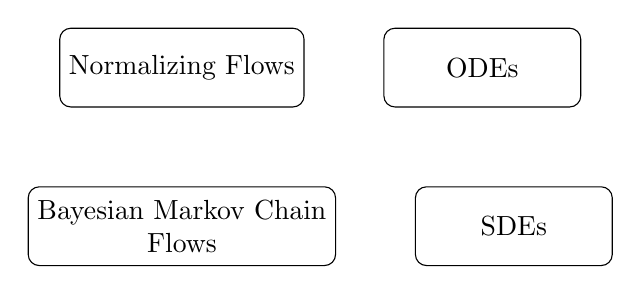
\begin{tikzpicture}[
        every node/.style={draw, align=center, rounded corners, minimum width=2.5cm, minimum height=1cm},
        arrow/.style={->, thick}
    ]
    
    % Nodes
    \node (norm) {Normalizing Flows};
    \node [right=of norm]  (ode) {ODEs};
    \node [below=of norm]  (markov) {Bayesian Markov Chain \\ Flows};
    \node [right=of markov]  (sde) {SDEs};

    
    % Arrows
    % \draw[arrow] (bijective) -- (injective);
    % \draw[arrow] (bijective) -- (stochastic);
    % \draw[arrow] (stochastic) -- (discrete);
    % \draw[arrow] (stochastic) -- (continuous);
    % \draw[arrow] (bijective) -- (incomp);

    
    \end{tikzpicture}
\end{center} 


Diffusion is basically infinitesimal compositions.

\subsection{Discrete Flows}

\subsection{Continuous Flows}

You can repres

\begin{align}
    \vx_0 \sim p_0; \quad d\vx_t &= U_t^{\theta}(\vx_t) dt &&\eqcomment{Flow Model} \\
    \vx_0 \sim p_0; \quad d\vx_t &= U_t^{\theta}(\vx_t) dt + \sigma_t dW_t && \eqcomment{Diffusion Model}
\end{align}


\section{Modelling Flows via Differential Equations}

\subsection{Stochastic Differential Equations}
Stochastic differential equations (SDEs) are the continuous counterpart of Markov chains, in the same way
as diffusion by ordinary differential equations is the continuous version of normalizing flows.

\section{Diffusion Models}

\begin{algorithm}
    \caption{Euler-Maruyama Method for Sampling from Diffusion Models}\label{alg:diff_sample}
    \begin{algorithmic}[1]
    \Require (Trained) Neural network $U_t^{\theta}$, diffusion coefficient $\sigma_t$
    \State Set $t \gets 0$
    \State Initialize the step size $h = 1 / N$
    \State Draw a sample from the initial distribution $\vx \sim p_0(\vx)$
    \For{$i = 1, \dots, N-1$}
    \State Draw sample $\epsilon \in \fN(0, I_D)$
    \State $\vx_{t+h} \gets \vx_t + h U_t^{\theta}(\vx_t) + \sigma_t \sqrt{h}\epsilon$
    \State Update time $t \gets t + h$
    \EndFor
    \State \Return $\vx_1$
    \end{algorithmic}
\end{algorithm}


\subsection{Architecture}
Earlier, the focus was on designing neural networks that were invertible - NICE, RealNVP, Invertible ResNetS, Glow.

\section{Latent Diffusion Models}

Latent Diffusion Models (LDMs) can be viewed as a development over another well-known class of generative models - Variational AutoEncoders (VAEs) \cite{dieleman2023perspectives}. It is pertinent to have a quick understanding of VAEs and how LDMs improve upon them.

VAEs are Bayesian Markov Flows.

How does ELBO relate to EBM? 



\subsection{Guidance}

\subsection{Sampling}


\section{Classifiers are Generative Models}

Optimizing = Gradient Descent
Sampling = Gradient Descent + noise
Guidance = ?

Since a generic classifier is not invertible, SGLD is a standard way of sampling from the distribution.

\section{Practical Aspects}

\section{Connections}
\subsection{Link between EBMs and Diffusion Models}
\subsection{Link between Neural ODEs and Diffusion Models}
\subsection{Link between SDG and SGLD}
\subsection{Link between Gaussian Processes and SDEs}

\appendix
\section{Mathematical Background}
\subsection{Probability Theory}


\bibliographystyle{unsrtnat} 
\bibliography{references}

\end{document}